\section{Stability Analysis}\label{stab}
\subsection{Preliminaries}
For the stability analysis of the fractional order system, the following theorem and definition, proposed and proved in \cite{abd2010chaos}, were applied:
\theoremstyle{definition}
\begin{definition}\label{def:1}
	Given a nonlinear differential system
    \begin{equation}
    	_CD_{0,t}^px(t)=f(x(t)),\quad x(t)\in\mathbb{R}^n
    \end{equation}
    where $x(0)=x_0$, $f(x)$ is continuous, the point $e$ is an equilibrium point of this system, if and only if $f(e)=0$.
\end{definition}
\begin{theorem}\label{theo:1}
Let $x=x^*$ be an equilibrium point of a fractional nonlinear system
\begin{equation}
D^\alpha x = f(x),\quad 0<\alpha<2
\end{equation}
If the eigenvalues of the Jacobian matrix $A = \partial f/\partial x|_{x=x^*}$ satisfy
\begin{equation}
 \min_{i}\left|\arg(\lambda_i)\right|>\alpha \frac{\pi}{2},\quad i=1,2,\dots,n.
\end{equation}
then $x^*$ is asymptotically stable.
\end{theorem}

\subsection{Results}
Analyzing the system shown in \ref{eq:main} and applying the definition \ref{def:1}, the equilibrium points are:
\begin{equation}
	\begin{array}{ll}
		p_1:&X=0\quad Y=\dfrac{1}{b}\quad Z=0\\
    	p_{2,3}:&X=\pm\sqrt{\dfrac{c-b-abc}{c}}\quad Y=\dfrac{1-x^2}{b}\quad Z=-\dfrac{x}{c}\\
	\end{array}
\end{equation}
Now, to analyze the stability of these equilibrium points, the Jacobian of the state variables is needed, thus
\begin{equation}
	J = \left[\begin{array}{ccc}
	Y-a &\quad X 	&\quad 1\\ 
    -2X 	&\quad -b 	&\quad 0\\
    -1 		&\quad 0 	&\quad c
	\end{array}\right]
\end{equation}

For the following simulations, the values for $a$, $b$ and $c$ will be, respectively, $3$, $0.1$ and $1$; $q_1=q_2=q_3=\alpha$ and $0<\alpha<1$ is assumed as well. Therefore, to use theorem \ref{theo:1}, the eigenvalues of the Jacobian matrix are required; using $p_1$ and $p_{2,3}$ as analysis points, the stability will be determined:

With the given values, $p_1=(0,10,0)$ and then respective Jacobian matrix is
\begin{equation}
	J_{p_1} = \left[\begin{array}{ccc}
	7 &\quad 0 	&\quad 1\\ 
    0 	&\quad -0.1		&\quad 0\\
    -1 		&\quad 0 	&\quad -1
	\end{array}\right]
\end{equation}
with eigenvalues $\lambda_1=-0.1$, $\lambda_2\approx 6.8730$ and $\lambda_3\approx-0.8730$. Now, theorem \ref{theo:1} is applied, $\min|\arg(\lambda_1),\arg(\lambda_2),\arg(\lambda_3)|=\min|\pi,\pi,0|=0<\alpha\frac{\pi}{2}$ since $0<\alpha<1$; therefore, according to the theorem, $p_1$ is an unstable equilibrium point.

Following a similar procedure for $p_{2,3}$, it can be obtained that the eigenvalues are $\lambda_1\approx-0.7256$, $\lambda_2\approx0.3128-1.2474i$ and $\lambda_3\approx0.3128+1.2474i$. In this case, we shall analyze the order of the fractional differential equation system ($\alpha$). Given \begin{equation*}
	\min_i|\arg(\lambda_i)|>\alpha\frac{\pi}{2}
\end{equation*}
It can solved for $\alpha$ and obtain a critical value for the order, hence
\begin{equation}
	\alpha < \frac{2}{\pi}\min_i|\arg(\lambda_i)|
\end{equation}
In this case, $\alpha <\frac{2}{\pi}\min_i|\arg(\lambda_1),\arg(\lambda_2),\arg(\lambda_3)| = \frac{2}{\pi}(1.3251)\approx0.8436$. Therefore, if $\alpha<0.8436$ the point $p_{2,3}$ is asymptotically stable; in any other case, is unstable.



\section{Control}
\subsection{Preliminaries}
It is desired to stabilize the system \ref{eq:main} in a periodic orbit (or in a fixed point) $\left(\tilde{x},\tilde{y},\tilde{z}\right)$ using feedback control, as in \cite{abd2010chaos}, hence
\begin{equation}
\begin{array}{ll}
\dfrac{d^{q_1}X}{dt^{q_1}}&=Z+(Y-a)X+u_1(t)\\
\dfrac{d^{q_2}Y}{dt^{q_2}}&=1-bY-X^2+u_2(t)\\
\dfrac{d^{q_3}Z}{dt^{q_3}}&=-X-cZ+u_3(t)\\
\end{array}
\end{equation}

Following the procedure described in \cite{abd2010chaos}, the control functions are defined by
\begin{equation}
	\begin{array}{ll}
		u_1(t)&=-(xy-\tilde{x}\tilde{y})\\
        u_2(t)&=x^2-\tilde{x}^2\\
        u_3(t)&=x-\tilde{x}
	\end{array}
\end{equation}

\subsection{Results}
\subsubsection{Stabilizing the system to a periodic orbit}
For the following simulations, $\alpha=0.9$ will be used. Additionally, the same values from section \ref{stab} for $a$, $b$ and $c$ are used. The solution to the system was obtained with the same Adams-Bashforth-Moulton predictor-corrector, with $N=3000$ and $T=300$. 
	\begin{figure}[H]
        \centering
        \begin{subfigure}[b]{0.475\textwidth}
            \centering
            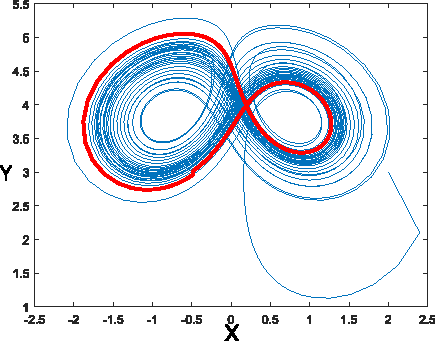
\includegraphics[scale=0.75]{files/OrbitXvsYq0_9.pdf}
            \caption{Uncontrolled phase plane for $XY$ with selected orbit.}    
            \label{fig:unctrlXY}
        \end{subfigure}
        \hfill
        \begin{subfigure}[b]{0.475\textwidth}  
            \centering 
            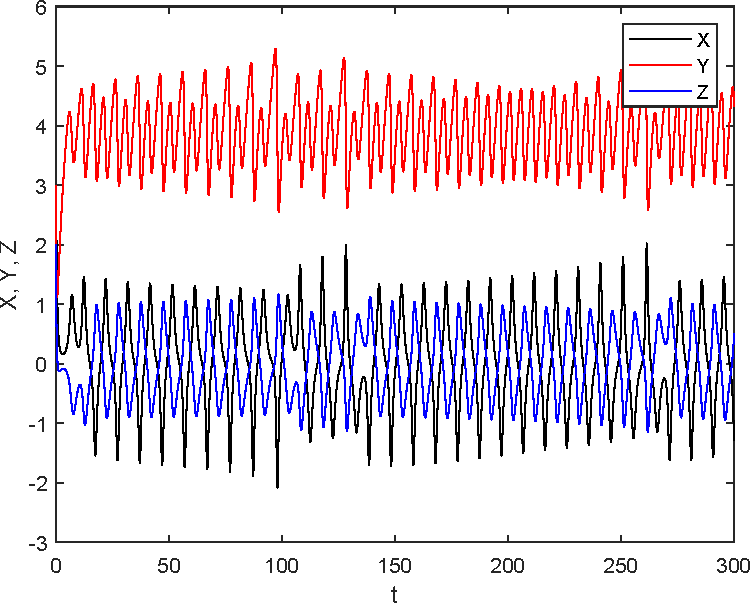
\includegraphics[scale=0.5]{files/OrbitXYZq0_9.pdf}
            \caption{Uncontrolled XYZ against time.}  
            \label{fig:unctrlXYZ}
        \end{subfigure}
        \vskip\baselineskip
        \begin{subfigure}[b]{0.475\textwidth}   
            \centering 
            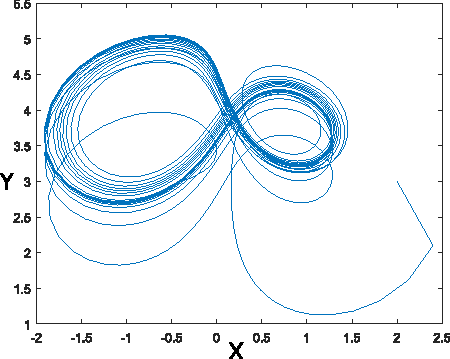
\includegraphics[scale=0.75]{files/ctrlXvsYq0_97.pdf}
            \caption{Controlled phase plane for $XY$.}    
            \label{fig:ctrlXY}
        \end{subfigure}
        \quad
        \begin{subfigure}[b]{0.475\textwidth}   
            \centering 
            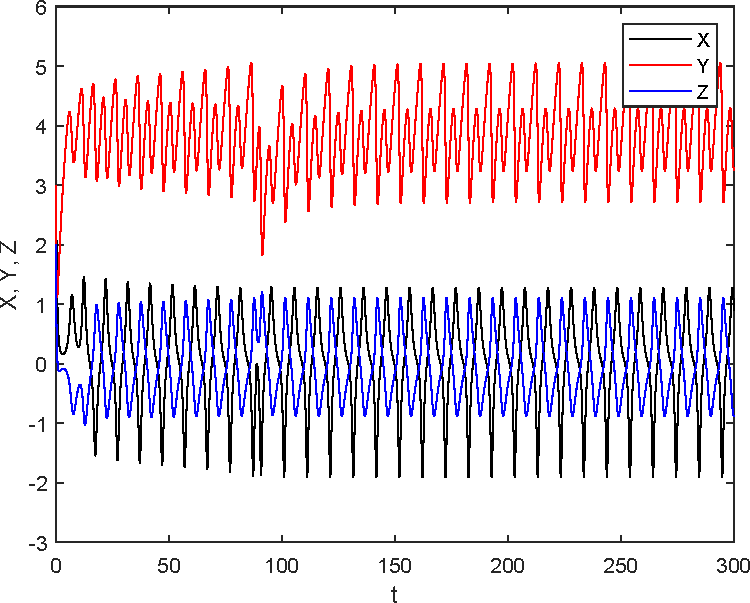
\includegraphics[scale=0.5]{files/ctrlorbitXYZq0_97.pdf}
            \caption{Controlled XYZ against time.}  
            \label{fig:ctrlXYZ}
        \end{subfigure}
        \caption{Results for controlled system in the selected orbit.} 
        \label{fig:o1}
	\end{figure}
      In figure \ref{fig:unctrlXY}, the red path is the selected periodic orbit to stabilize. The period of said orbit is $10.2$, the interval for it is $[78.2,88.4]$. On figure \ref{fig:unctrlXYZ}, the behavior of the state variables through time is shown, note the periodic behavior of these variables through time after the control is applied.
    
    In figure \ref{fig:o1}(a-b), the response for the proposed control is shown. The controller starts when the system fully completes the selected orbit (i.e $t=88.4$), in order to ensure that it remains in a similar shape. Before applying the feedback control, $u_i(t)=0$, $i=1,2,3$. Note that the response is periodic and more consistent compared to the original.

\subsubsection{Stabilizing the system to a fixed point}
In this section, the same $\alpha$, $a$, $b$ and $c$ are used as in the previous simulations, except for the last plot (i.e figure \ref{img:p2}) that $\alpha=0.95$. In order to obtain these results, the controller starts working at $t=22.5$. 
\begin{figure}[H]
  \centering
  \begin{subfigure}[H]{0.4\textwidth}
    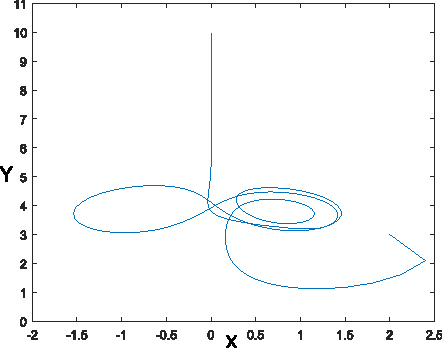
\includegraphics[scale = 0.75]{files/ctrlxvsYFixed0_9.pdf}
    \centering
    \caption{Phase plane for $XY$.}
    \label{fig:p1fixedxy}
  \end{subfigure}
  \hspace{1cm}
  \begin{subfigure}[H]{0.4\textwidth}
    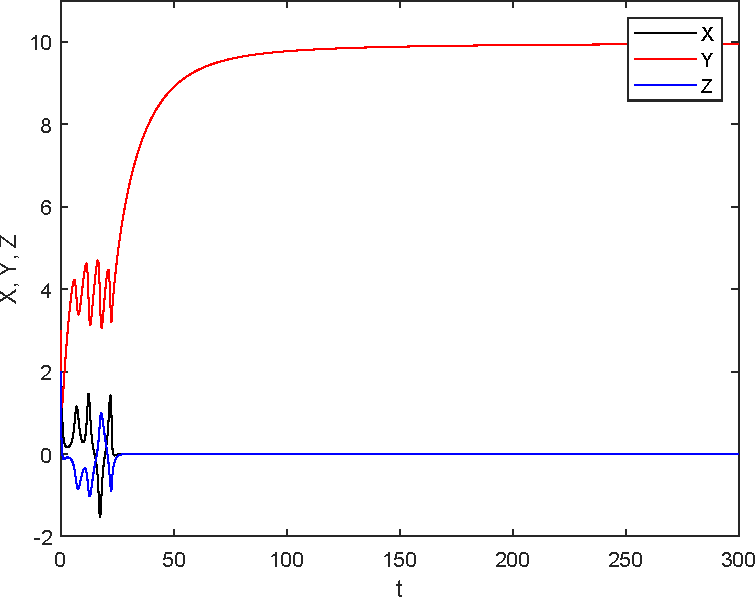
\includegraphics[scale = 0.5]{files/ctrlq0_9.pdf}
    \centering
    \caption{$XYZ$ against time.}
    \label{fig:p1fixedxyz}
  \end{subfigure}
  \caption{Results for controlled system around $p_1$.}
  \label{img:p1}
\end{figure}
In figure \ref{img:p1}, the stabilization for the equilibrium point $p_1=(0,10,0)$ is exhibited. The figure on the left shows how the system converges to this point. The figure on the right shows the behavior of the states variables through time, showing that they also converge to $p_1$.
\begin{figure}[H]
  \centering
  \begin{subfigure}[H]{0.4\textwidth}
    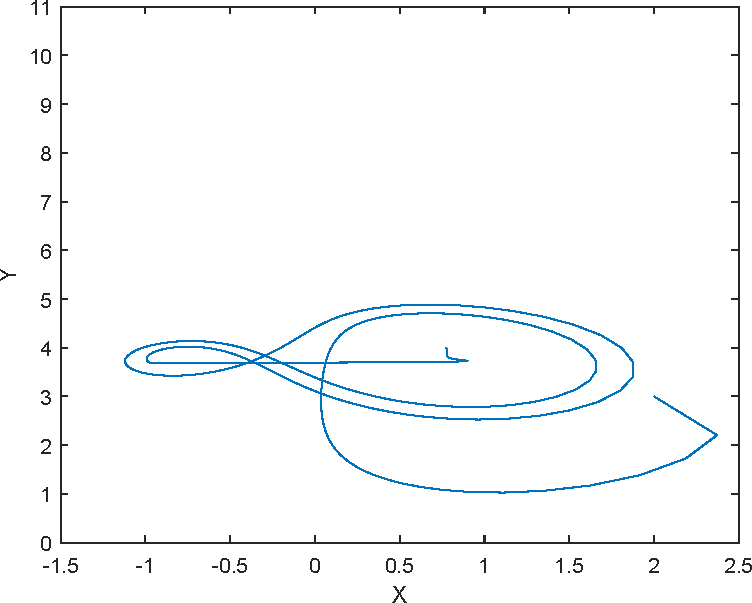
\includegraphics[scale = 0.5]{files/ctrlXvsYFixedq0_95.pdf}
    \centering
    \caption{Phase plane for $XY$.}
    \label{fig:p2fixedxy}
  \end{subfigure}
  \hspace{1cm}
  \begin{subfigure}[H]{0.4\textwidth}
    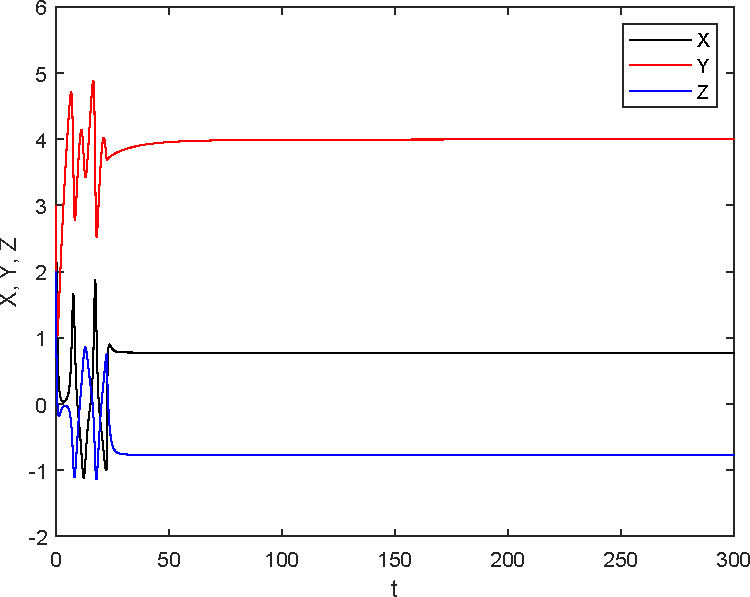
\includegraphics[scale = 0.5]{files/ctrlq0_95.pdf}
    \centering
    \caption{$XYZ$ against time.}
    \label{fig:p2fixedxyz}
  \end{subfigure}
  \caption{Results for controlled system around $p_2$.}
  \label{img:p2}
\end{figure}
In figures \ref{img:p2}(a-b), the equilibrium is achieved around $p_2$, using the same procedure as in the previous simulation. Note that $\alpha=0.95$.

The results obtained in this section can be compared with fixed-point stabilization in Abd-Elouahab \textit{et al.} in \cite{abd2010chaos}.

It can be seen that the system is highly controllable, through the feedback control methodology presented in \cite{abd2010chaos}. There are others types of controllers proposed in the literature for this fractional-order system; see \cite{pan2015multi} or \cite{yang2017modified}.




